% begin module velocity-ex3
\begin{frame}
\frametitle{Velocities}
\begin{example} %[Example 3, p. 137]
Suppose a ball is dropped from the upper deck of the CN Tower, 450m above the ground.  What is the velocity of the ball after 5 seconds?
\end{example}
\begin{itemize}
\item<2->  We need to know what ``instantaneous'' velocity is.
\item<3->  Let $f(x)$ denote the displacement of an object at time $x$.
%\item<4->  The slope of the secant from $(a, f(a))$ to $(x, f(x))$ is the average velocity over the interval $[a, x]$.
%\item<5->  The slope of the tangent line at $a$ is the instantaneous velocity at the time $a$.
\end{itemize}
\begin{center}
\begin{columns}[c]
\column{.4\textwidth}
\ \uncover<4->{%

\psset{xunit=0.5cm, yunit=0.5cm}
\begin{pspicture}(-1,-1.5)(5.4,4.6)
\psframe*[linecolor=white](-1,-1.5)(5.4,4.6)
\psaxes[ticks=none, labels=none]{<->}(0,0)(-1,-1.5)(5.4,4.6)
%Function formula: -11/8+5/18 ((x) ((x) (x)))-1/81 ((x) ((x) ((x) (x))))-73/36 ((x) (x))+43/8 (x)
\psplot[linecolor=red, plotpoints=1000]{0}{5}{x 5.375 mul x x mul -2.02778 mul add x x mul x mul x mul -0.0123457 mul add x x mul x mul 0.277778 mul add -1.375 add }

\fcFullDotBlack{0.5}{0.839506173}

\rput[rb] (0.6,0.92){\tiny$P=(a, f(a))$}
\rput[t](0.5, -0.1){\tiny$a$}
\psline(0.5,0.1)(0.5,0)

\psline[linestyle=dashed](0.5, 0)(0.5, 0.839506173)

\psline[linecolor=blue](0, 0.631173)(5, 2.71451)
\fcFullDotBlack{4}{2.29784}
\psline[linestyle=dashed](4, 0)(4, 2.29784)
\psline(0.5, 0.839506173)(4,0.839506173) (4, 2.29784)
\rput[t](4, -0.1){\tiny$x$}
\rput[l](4.1, 1.5){\tiny$f(x)-f(a)$}
\rput[t](2.25, 0.82){\tiny$x-a$}
\rput[b](4, 4){\tiny $Q=(x,f(x))$}
\psline[linestyle=dotted]{->}(4,3.9)(4, 2.29784)
\end{pspicture}
%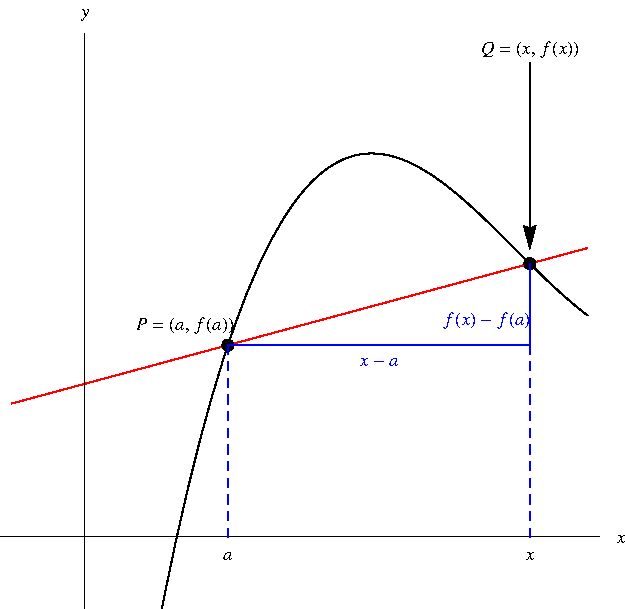
\includegraphics[height=3.5cm]{derivatives/pictures/03-01-secanta.pdf}%

Slope of secant\\ $ = $ average velocity
}%
\column{.4\textwidth}
\ \uncover<5->{%
\psset{xunit=0.5cm, yunit=0.5cm}
\begin{pspicture}(-1,-1.5)(5.4,4.6)
\psframe*[linecolor=white](-1,-1.5)(5.4,4.6)
\psaxes[ticks=none, labels=none]{<->}(0,0)(-1,-1.5)(5.4,4.6)
%Function formula: -11/8+5/18 ((x) ((x) (x)))-1/81 ((x) ((x) ((x) (x))))-73/36 ((x) (x))+43/8 (x)
\psplot[linecolor=red, plotpoints=1000]{0}{5}{x 5.375 mul x x mul -2.02778 mul add x x mul x mul x mul -0.0123457 mul add x x mul x mul 0.277778 mul add -1.375 add }

\psline[linecolor=blue](0, -0.935185185)(1.531304348, 4.5)
\fcFullDotBlack{0.5}{0.839506173}

\rput[rb] (0.6,0.92){\tiny$P=(a, f(a))$}
\rput[t](0.5, -0.1){\tiny$a$}
\psline(0.5,0.1)(0.5,0)
\end{pspicture}
%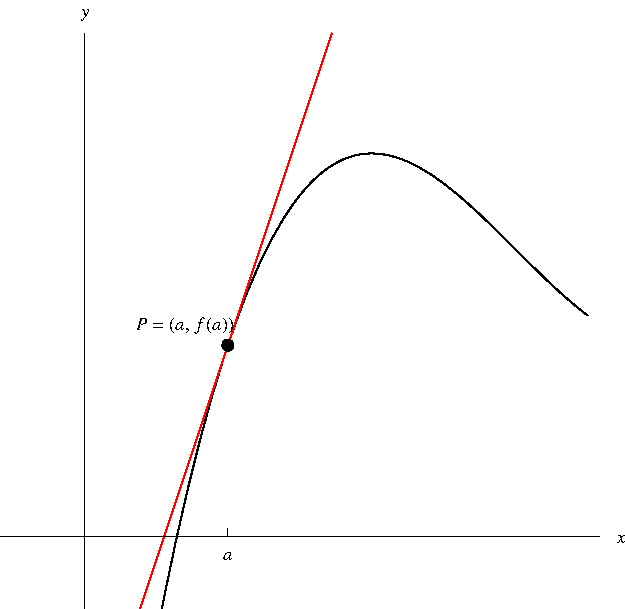
\includegraphics[height=3.5cm]{derivatives/pictures/03-01-tangent.pdf}%

Slope of tangent\\ $ = $ instantaneous velocity
}%
\end{columns}
\end{center}
\end{frame}

\begin{frame}
\begin{example} %[Example 3, p. 137]
Suppose a ball is dropped from the upper deck of the CN Tower, 450m above the ground.  What is the velocity of the ball after 5 seconds?
\begin{itemize}
\item<2->  The distance $f(x)$ (in meters) that the ball has fallen at time $x$ (in seconds) follows Galileo's law: $f(x) = 4.9x^2$.
\item<3->  Let $v(a)$ be its velocity at time $a$.
\end{itemize}
\abovedisplayskip=0pt
\belowdisplayskip=0pt
\begin{align*}
\uncover<4->{%
v(a)
}%
& \uncover<4->{ = } %
\uncover<4->{%
\lim_{h\rightarrow 0}\frac{f(a+h)-f(a)}{h}
}  \uncover<5->{ = } \uncover<5->{%
\lim_{h\rightarrow 0}\frac{4.9(a+h)^2-4.9a^2}{h}
}\\%
& \uncover<6->{ = } %
\uncover<6->{%
\lim_{h\rightarrow 0}\frac{4.9(a^2+2ah+h^2)-4.9a^2}{h}
}\\%
& \uncover<7->{ = } %
\uncover<7->{%
\lim_{h\rightarrow 0}\frac{4.9(2ah+h^2)}{h}
}\\%
& \uncover<8->{ = } %
\uncover<8->{%
\lim_{h\rightarrow 0}4.9(2a+h)
}%
\uncover<9->{%
 = 9.8a
}%
\end{align*}
\uncover<10->{%
Therefore the velocity after 5s is $v(5) = 9.8(5) = 49$m/s.
}%
\end{example}
\end{frame}
% end module velocity-ex3
